\documentclass[aspectratio=169]{beamer}

\mode<presentation>
{
  \usetheme{default}
  \usecolortheme{default}
  \usefonttheme{default}
  \setbeamertemplate{navigation symbols}{}
  \setbeamertemplate{caption}[numbered]
  \setbeamertemplate{footline}[frame number]  % or "page number"
  \setbeamercolor{frametitle}{fg=white}
  \setbeamercolor{footline}{fg=black}
} 

\usepackage[english]{babel}
\usepackage[utf8x]{inputenc}
\usepackage{tikz}
\usepackage{courier}
\usepackage{array}
\usepackage{bold-extra}
\usepackage{minted}
\usepackage[thicklines]{cancel}

\xdefinecolor{dianablue}{rgb}{0.18,0.24,0.31}
\xdefinecolor{darkblue}{rgb}{0.1,0.1,0.7}
\xdefinecolor{darkgreen}{rgb}{0,0.5,0}
\xdefinecolor{darkgrey}{rgb}{0.35,0.35,0.35}
\xdefinecolor{darkorange}{rgb}{0.8,0.5,0}
\xdefinecolor{darkred}{rgb}{0.7,0,0}
\definecolor{darkgreen}{rgb}{0,0.6,0}
\definecolor{mauve}{rgb}{0.58,0,0.82}

\title[2018-04-30-paris-oamap]{Object-array mapping and columnar data granularity}
\author{Jim Pivarski}
\institute{Princeton University -- DIANA-HEP}
\date{April 30, 2018}

\begin{document}

\logo{\pgfputat{\pgfxy(0.11, 7.4)}{\pgfbox[right,base]{\tikz{\filldraw[fill=dianablue, draw=none] (0 cm, 0 cm) rectangle (50 cm, 1 cm);}\mbox{\hspace{-8 cm}\includegraphics[height=1 cm]{princeton-logo-long.png}\includegraphics[height=1 cm]{diana-hep-logo-long.png}}}}}

\begin{frame}
  \titlepage
\end{frame}

\logo{\pgfputat{\pgfxy(0.11, 7.4)}{\pgfbox[right,base]{\tikz{\filldraw[fill=dianablue, draw=none] (0 cm, 0 cm) rectangle (50 cm, 1 cm);}\mbox{\hspace{-8 cm}\includegraphics[height=1 cm]{princeton-logo.png}\includegraphics[height=1 cm]{diana-hep-logo.png}}}}}

% Uncomment these lines for an automatically generated outline.
%\begin{frame}{Outline}
%  \tableofcontents
%\end{frame}

% START START START START START START START START START START START START START

\begin{frame}{Context}
\vspace{0.35 cm}
\begin{columns}[t]
\column{0.4\linewidth}
\underline{High Performance Computing (HPC)}

\vspace{0.15 cm}
\begin{itemize}
\item A lot of focus on data contiguity, CPU cache efficiency, and vectorization.
\item Data structures are often converted to flat arrays or tables, making it easier to reason about such issues.
\end{itemize}

\column{0.56\linewidth}
\begin{uncoverenv}<2->
\underline{High Energy Physics (HEP)}

\vspace{0.15 cm}
\begin{itemize}
\item Data structures are generally:

\begin{center}
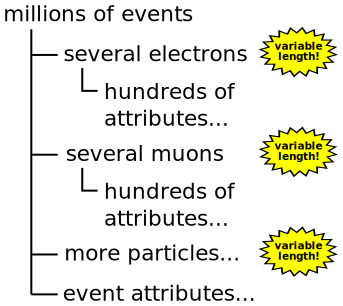
\includegraphics[width=0.7\linewidth]{event-structure.pdf}
\end{center}

\item Analysis code is branchy and pointer-heavy;

``Looks more like string processing!''
\end{itemize}
\end{uncoverenv}
\end{columns}
\end{frame}

\begin{frame}{Context}
\vspace{0.5 cm}
Preparing data for analysis consists of {\it copying} parts of the centrally produced dataset.

\vspace{0.25 cm}
The choice of events to ``skim'' and which attributes to ``slim'' has to be decided before interactive data exploration is possible (timescale of seconds).

\vspace{0.5 cm}
\begin{columns}[c]
\column{0.5\linewidth}
\mbox{ } \hfill \includegraphics[height=4.5 cm]{cms-data-explosion.png}

\column{0.5\linewidth}

\vspace{0.2 cm}
\includegraphics[height=4.4 cm]{atlas-data-explosion.png} \hfill \mbox{ }
\end{columns}
\end{frame}

\begin{frame}{Context}
\vspace{0.5 cm}
It's the data structures and code branchiness that are preventing HEP from taking advantage of HPC techniques.

\vspace{0.25 cm}
\begin{itemize}\setlength{\itemsep}{0.5 cm}
\item[$\rightarrow$]<2-> Several projects underway to rewrite or rethink core reconstruction algorithms: vectorized tracking, machine learning-based pattern recognition\ldots

\item[$\rightarrow$]<3-> But a substantial part is post-reconstruction data analysis.
\begin{itemize}\setlength{\itemsep}{0.1 cm}
\item<4-> not centrally produced: ``users'' of the data
\item<5-> ad-hoc (``if we knew what we were doing, it wouldn't be called research'')
\item<6-> sometimes egregiously inefficient\ldots
\end{itemize}
\end{itemize}
\end{frame}

\begin{frame}{New technique}
\vspace{0.5 cm}
\textcolor{darkblue}{\large \underline{Object-array mapping (OAMap)}}

\vspace{0.25 cm}
\begin{itemize}\setlength{\itemsep}{0.25 cm}
\item Let data analysts write traditional object-oriented code, but translate it to HPC-like array operations at runtime. (Generalization of AOS$\to$SOA.)
\item<2-> Analogy with object-relational mapping (ORM), but for low-level arrays.
\item<3-> Represent nested, variable-length object data as (unequal length) arrays of each attribute and {\it never deserialize} it into runtime objects.
\item<4-> Two ways of implementing it:

\vspace{0.05 cm}
\begin{description}\setlength{\itemsep}{0.1 cm}
\item[proxies]<5-> that simulate objects on the fly by accessing array data in response to attribute references (low-latency exploration).
\item[compiled]<6-> form that eliminates all objects, even temporary proxies, replacing user code with code that accesses array elements directly.
\end{description}
\end{itemize}
\end{frame}



\end{document}
